\section{Context: Polarization and the Poincar\'e sphere}
\subsection{Linked representations}

\begin{frame}{Jones vectors and the Poincar\'e sphere}
\begin{columns}[T,onlytextwidth]
\column{0.60\textwidth}
For a normalized, fully polarized state,
\[
\mathbf J=\begin{pmatrix}a\\b\,e^{i\varphi}\end{pmatrix},
\qquad a,b\geq0,\quad a^2+b^2=1.
\]
The applet uses
\[
\mathbf S=\begin{pmatrix}
a^2-b^2\\2ab\cos\varphi\\2ab\sin\varphi
\end{pmatrix},\qquad \lVert\mathbf S\rVert=1,
\]
Polarization is a valid approach to introductory quantum computing \citep{15rm-rlnj}.
% akin to a Qubit on the Bloch sphere, \(\ket{\psi}=\cos\frac{\vartheta}{2}\ket{0}+e^{i\varphi}\sin\frac{\vartheta}{2}\ket{1}\), 


\column{0.40\textwidth}
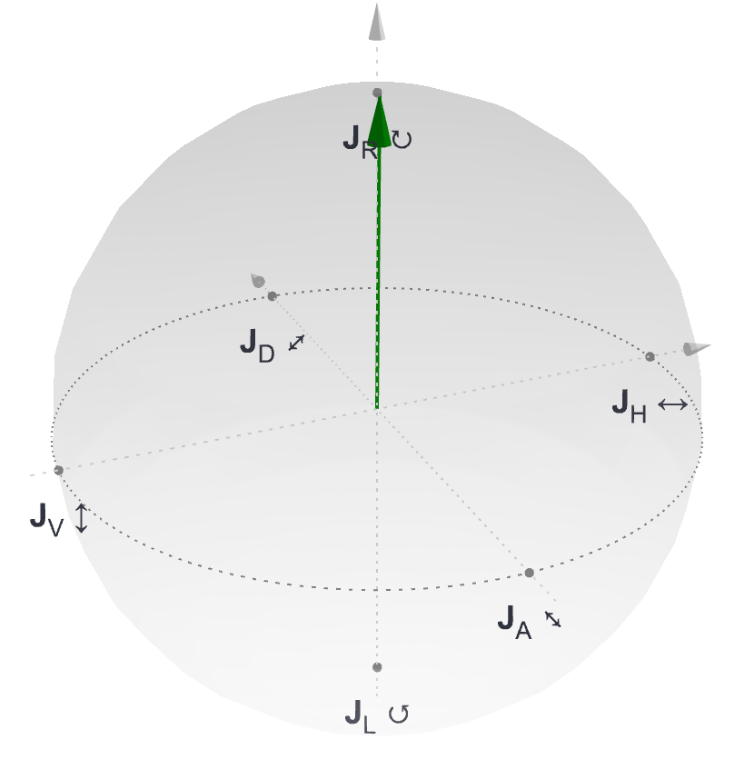
\includegraphics[width=\textwidth]{images/poincare.png}
\end{columns}
\vspace{2mm}
% \textbf{A point denotes a polarization state, not a position in the laboratory.}
% \source{Equations and labels follow the applet's convention.}
\slidesource{Polarization applet Github \citep{2026polarization}}
\note{With standard Pauli-matrix ordering for the same two-component state, the Bloch vector is (S2,S3,S1). Circular-polarization names depend on propagation and phase conventions. Keep the applet's convention throughout the presentation.}
\end{frame}

%\begin{frame}{What the geometric connection does and does not show}
%\begin{itemize}
%\item After choosing a basis and axis convention, pure qubit states and normalized Jones states share the same sphere geometry.
%\item An overall phase does not change the represented state.
%\item A lossless wave plate changes the state without reducing intensity.
%\item A polarizer changes the transmitted state and usually reduces intensity. The sphere alone does not encode that intensity.
%\end{itemize}
%\keyidea{The teaching challenge is interpreting a mathematical state space without turning it into a literal physical object.}
%\source{Jones-calculus implementation and the teaching rationale.}
%\note{At zero transmitted intensity, a normalized output polarization state is undefined. Avoid using a sphere point to imply that an extinguished field has a measurable polarization. This presentation does not claim that classical polarization reproduces all quantum phenomena.}
%\end{frame}

\subsection{Conditions and tasks}
\begin{frame}{The applet}
\begin{columns}[T,onlytextwidth]
\column{0.48\textwidth}
\centering
\textbf{Control:} \\ Jones notation and spatial wave graph.
\column{0.48\textwidth}
\centering
\textbf{Experimental:} \\ Adding the Poincar\'e sphere.
\end{columns}
\centering
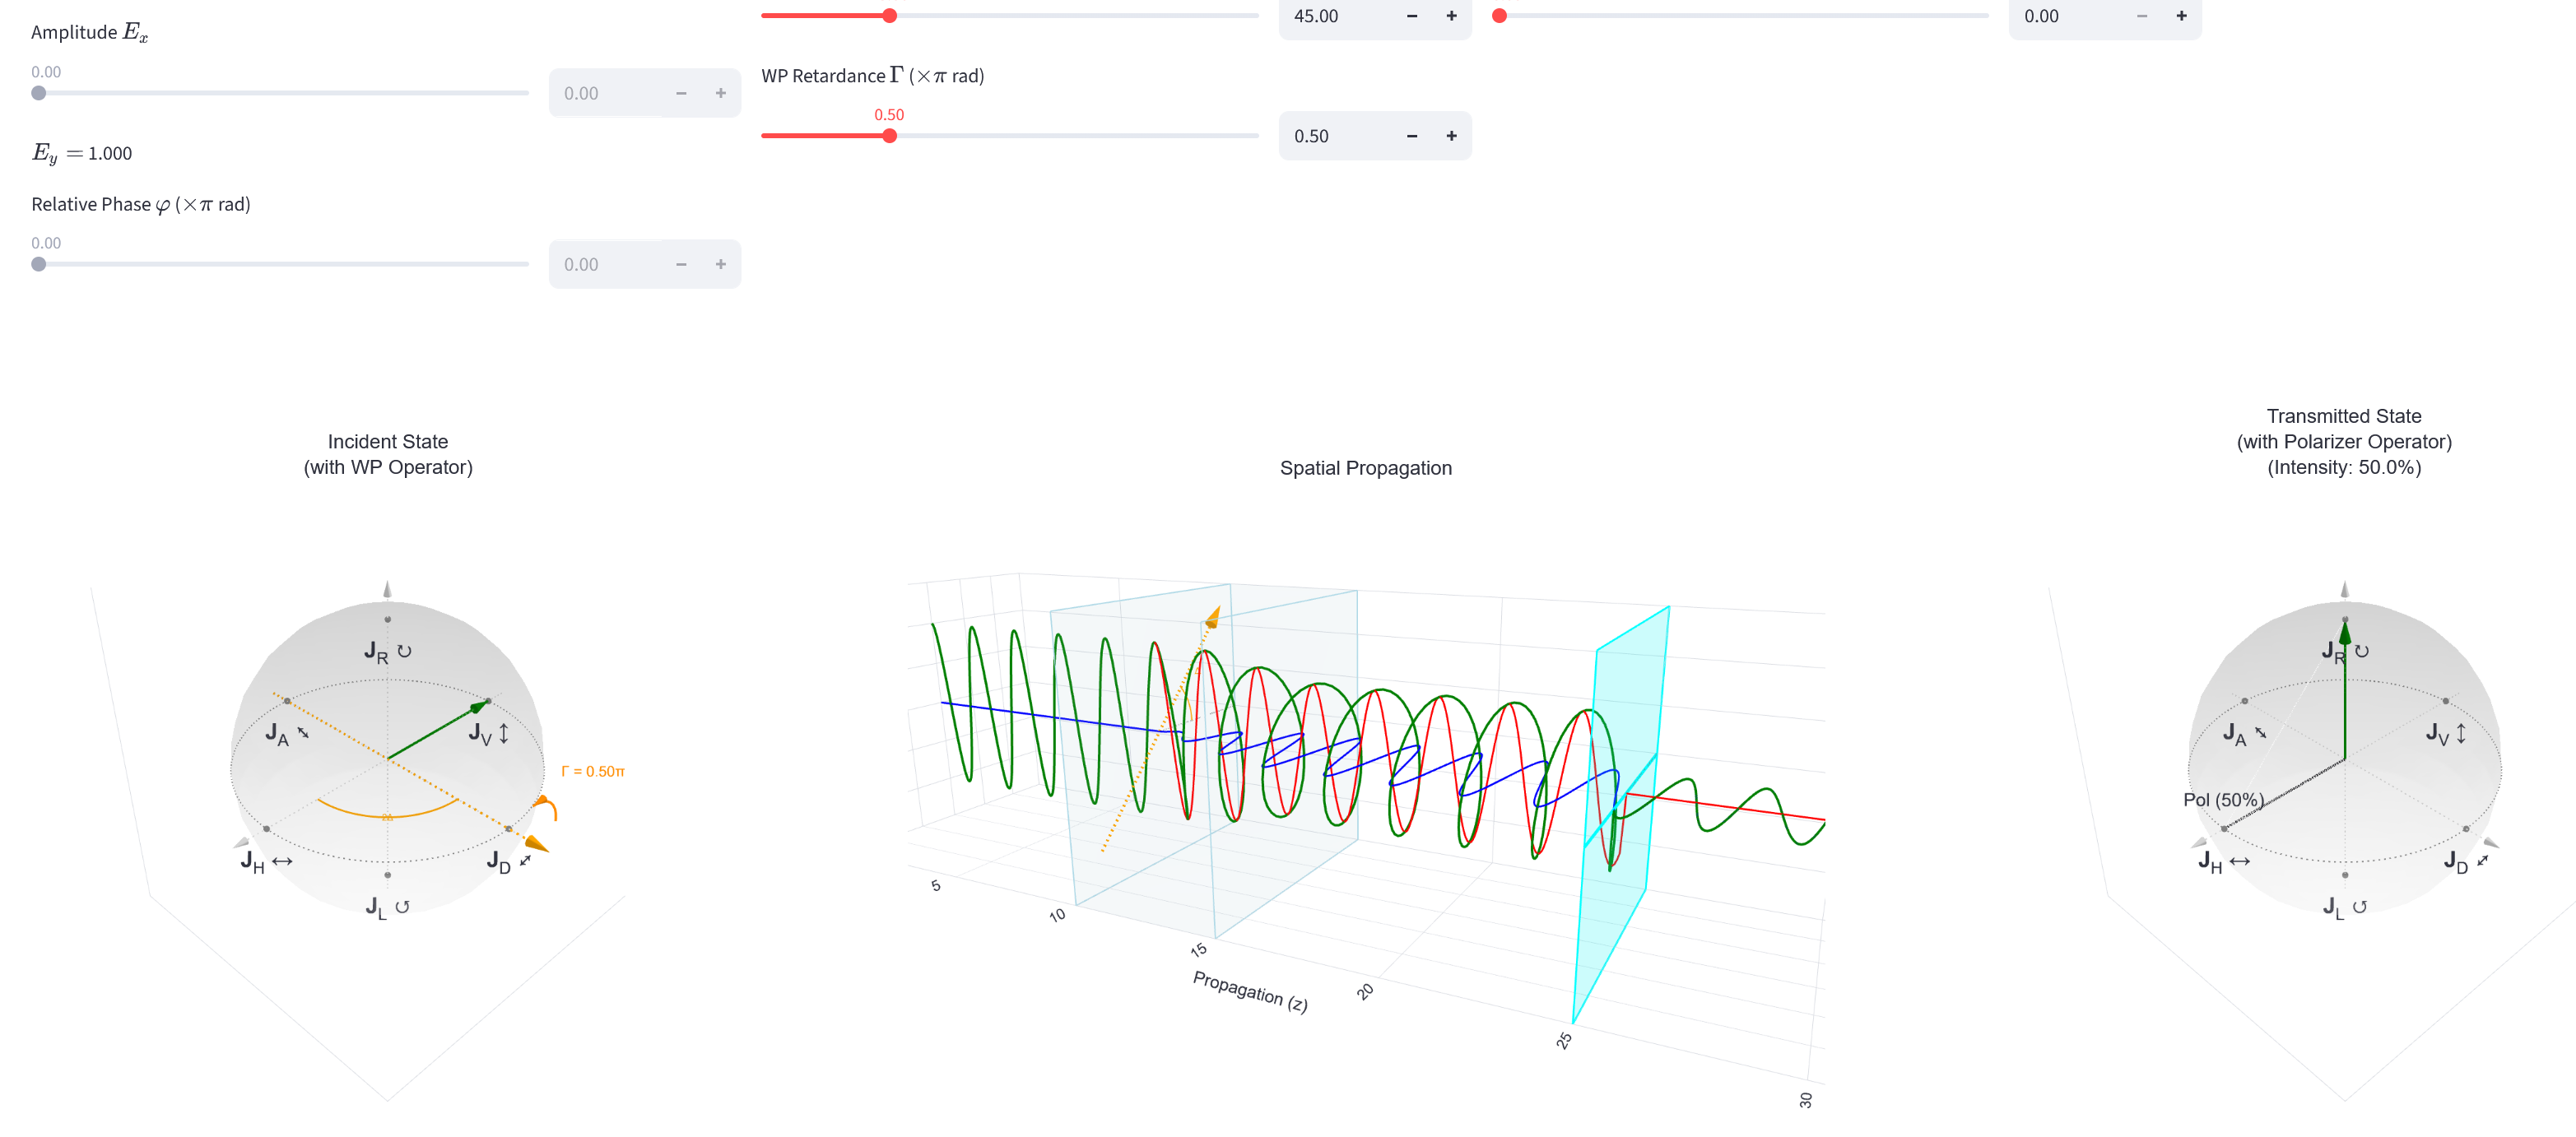
\includegraphics[width=0.85\textwidth]{images/applet.png}

+ Introductory explanations, guided parameter changes, hints, and solutions. 
% \source{Condition mapping and timing: \texttt{app.py} and \texttt{challenges.py}.}
\slidesource{Polarization applet Github \citep{2026polarization}}
\note{Use screenshots of the same optical state and step. The current versions also differ in instructional wording and one initial wave-plate angle. See the implementation appendix before describing the contrast as a purely visual manipulation.}
\end{frame}

\begin{frame}{The learning sequence}
\begin{tabularx}{\textwidth}{@{}P{0.13\textwidth}P{0.29\textwidth}Y@{}}
\toprule
\textbf{Steps} & \textbf{Topic} & \textbf{Learner activity} \\
\midrule
1--3 & Polarization states & Change amplitudes and relative phase to construct linear and circular states. \\
4--6 & Wave plates & Vary retardance and fast-axis orientation to transform a state. \\
7 & Linear polarizers & Relate transmission-axis orientation to output intensity. \\
8--9 & Combined operators & Coordinate wave plates and polarizers to meet a target. \\
\bottomrule
\end{tabularx}\par
\vspace{3mm}
Nine challenges precede a completion screen and survey return link.
% \source{Challenge definitions. A revealed solution can also satisfy the target.}
\end{frame}

